\paragraph{Unity}

В качестве фреймворка для выполнения проекта был выбран Unity.
Unity~--~это фреймворк, предназначенный для разработки интерактивных графических приложений.%
\cite{DocUnity}
Первая версия фреймворка была выпущена в 2005 году
и с тех пор продолжает активно развиваться.
Для создания приложений Unity поддерживает более 20 платформ,
включающих персональные компьютеры, мобильные устройства, игровые консоли и др.
Фреймворк может быть использован для создания приложений
с двумерной или трехмерной графикой, а также приложений
в виртуальной или дополненной реальности.

\begin{figure}[ht]
    \centering
    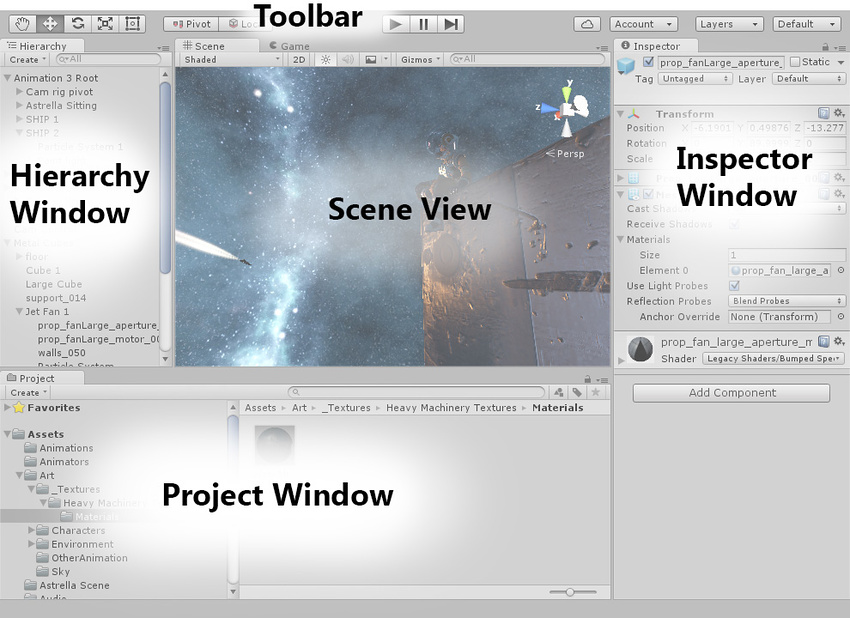
\includegraphics[width=0.9\textwidth, frame]{images/Unity-interface.jpg}
    \caption{Графический интерфейс редактора Unity.%
    \cite{DocUnity}}
    \label{figure:UnityInterface}
\end{figure}

Unity имеет встроенные модули для работы с
графикой, пользовательским вводом, физикой,
пользовательским интерфейсом и сетевым взаимодействием.
Компонентная архитектура фреймворка позволяет
легко расширять уже существующую функциональность.

Основное направление использования Unity -- это разработка игр,
тем не менее Unity также успешно применяется в киноиндустрии,\cite{UnityInFilmmaking}
архитектуре, автомобилестроении,\cite{UnityInAutomotive}
разработке виртуальных тренажеров, а также в
обучении искусственного интеллекта.\cite{UnityInAI}
